%%%%%%%%%%%%%%%%%%%%%%%%%%%%%%%%%%%%%%%%%
% Wenneker Assignment
% LaTeX Template
% Version 2.0 (12/1/2019)
%
% This template originates from:
% http://www.LaTeXTemplates.com
%
% Authors:
% Vel (vel@LaTeXTemplates.com)
% Frits Wenneker
%
% License:
% CC BY-NC-SA 3.0 (http://creativecommons.org/licenses/by-nc-sa/3.0/)
% 
%%%%%%%%%%%%%%%%%%%%%%%%%%%%%%%%%%%%%%%%%

%----------------------------------------------------------------------------------------
%	PACKAGES AND OTHER DOCUMENT CONFIGURATIONS
%----------------------------------------------------------------------------------------

\documentclass[11pt]{scrartcl} % Font size

%%%%%%%%%%%%%%%%%%%%%%%%%%%%%%%%%%%%%%%%%
% Wenneker Assignment
% Structure Specification File
% Version 2.0 (12/1/2019)
%
% This template originates from:
% http://www.LaTeXTemplates.com
%
% Authors:
% Vel (vel@LaTeXTemplates.com)
% Frits Wenneker
%
% License:
% CC BY-NC-SA 3.0 (http://creativecommons.org/licenses/by-nc-sa/3.0/)
% 
%%%%%%%%%%%%%%%%%%%%%%%%%%%%%%%%%%%%%%%%%

%----------------------------------------------------------------------------------------
%	PACKAGES AND OTHER DOCUMENT CONFIGURATIONS
%----------------------------------------------------------------------------------------

\usepackage{amsmath, amsfonts, amsthm} % Math packages

\usepackage{listings} % Code listings, with syntax highlighting

\usepackage[english]{babel} % English language hyphenation

\usepackage{graphicx} % Required for inserting images
\graphicspath{{Figures/}{./}} % Specifies where to look for included images (trailing slash required)

\usepackage{booktabs} % Required for better horizontal rules in tables

\numberwithin{equation}{section} % Number equations within sections (i.e. 1.1, 1.2, 2.1, 2.2 instead of 1, 2, 3, 4)
\numberwithin{figure}{section} % Number figures within sections (i.e. 1.1, 1.2, 2.1, 2.2 instead of 1, 2, 3, 4)
\numberwithin{table}{section} % Number tables within sections (i.e. 1.1, 1.2, 2.1, 2.2 instead of 1, 2, 3, 4)

\setlength\parindent{0pt} % Removes all indentation from paragraphs

\usepackage{enumitem} % Required for list customisation
\setlist{noitemsep} % No spacing between list items

%----------------------------------------------------------------------------------------
%	DOCUMENT MARGINS
%----------------------------------------------------------------------------------------

\usepackage{geometry} % Required for adjusting page dimensions and margins

\geometry{
	paper=a4paper, % Paper size, change to letterpaper for US letter size
	top=2.5cm, % Top margin
	bottom=3cm, % Bottom margin
	left=3cm, % Left margin
	right=3cm, % Right margin
	headheight=0.75cm, % Header height
	footskip=1.5cm, % Space from the bottom margin to the baseline of the footer
	headsep=0.75cm, % Space from the top margin to the baseline of the header
	%showframe, % Uncomment to show how the type block is set on the page
}

%----------------------------------------------------------------------------------------
%	FONTS
%----------------------------------------------------------------------------------------

\usepackage[utf8]{inputenc} % Required for inputting international characters
\usepackage[T1]{fontenc} % Use 8-bit encoding

\usepackage{fourier} % Use the Adobe Utopia font for the document

%----------------------------------------------------------------------------------------
%	SECTION TITLES
%----------------------------------------------------------------------------------------

\usepackage{sectsty} % Allows customising section commands

\sectionfont{\vspace{6pt}\centering\normalfont\scshape} % \section{} styling
\subsectionfont{\normalfont\bfseries} % \subsection{} styling
\subsubsectionfont{\normalfont\itshape} % \subsubsection{} styling
\paragraphfont{\normalfont\scshape} % \paragraph{} styling

%----------------------------------------------------------------------------------------
%	HEADERS AND FOOTERS
%----------------------------------------------------------------------------------------

\usepackage{scrlayer-scrpage} % Required for customising headers and footers

\ohead*{} % Right header
\ihead*{} % Left header
\chead*{} % Centre header

\ofoot*{} % Right footer
\ifoot*{} % Left footer
\cfoot*{\pagemark} % Centre footer

%----------------------------------------------------------------------------------------
%	PARAGRAPH
%----------------------------------------------------------------------------------------

\setlength{\parskip}{8pt}
 % Include the file specifying the document structure and custom commands

%----------------------------------------------------------------------------------------
%	TITLE SECTION
%----------------------------------------------------------------------------------------

\title{	
	\normalfont\normalsize
	\rule{\linewidth}{0.5pt}\\ % Thin top horizontal rule
	\vspace{20pt} % Whitespace
	{\huge Gofinge Note for EM algorithm}\\ % The assignment title
	\vspace{12pt} % Whitespace
	\rule{\linewidth}{2pt}\\ % Thick bottom horizontal rule
	\vspace{12pt} % Whitespace
}

\author{\LARGE Xiaoyang Wu} % Your name

\date{\normalsize February 21, 2019} % Today's date (\today) or a custom date

\begin{document}

\maketitle % Print the title

%----------------------------------------------------------------------------------------
%	 INTRODUCTION
%----------------------------------------------------------------------------------------

\section{Introduction to expectation-maximization(EM)  algorithm}

\subsection{An example of EM algorithm}

Let's start with an example from Chuong B Do \& Serafim Batzoglou‘s tutorial paper \textit{What is the expectation maximization algorithm?}, and I have saved the .pdf file of this paper in the \textit{material} folder.

\begin{figure}[h] % [h] forces the figure to be output where it is defined in the code (it suppresses floating)
	\centering
	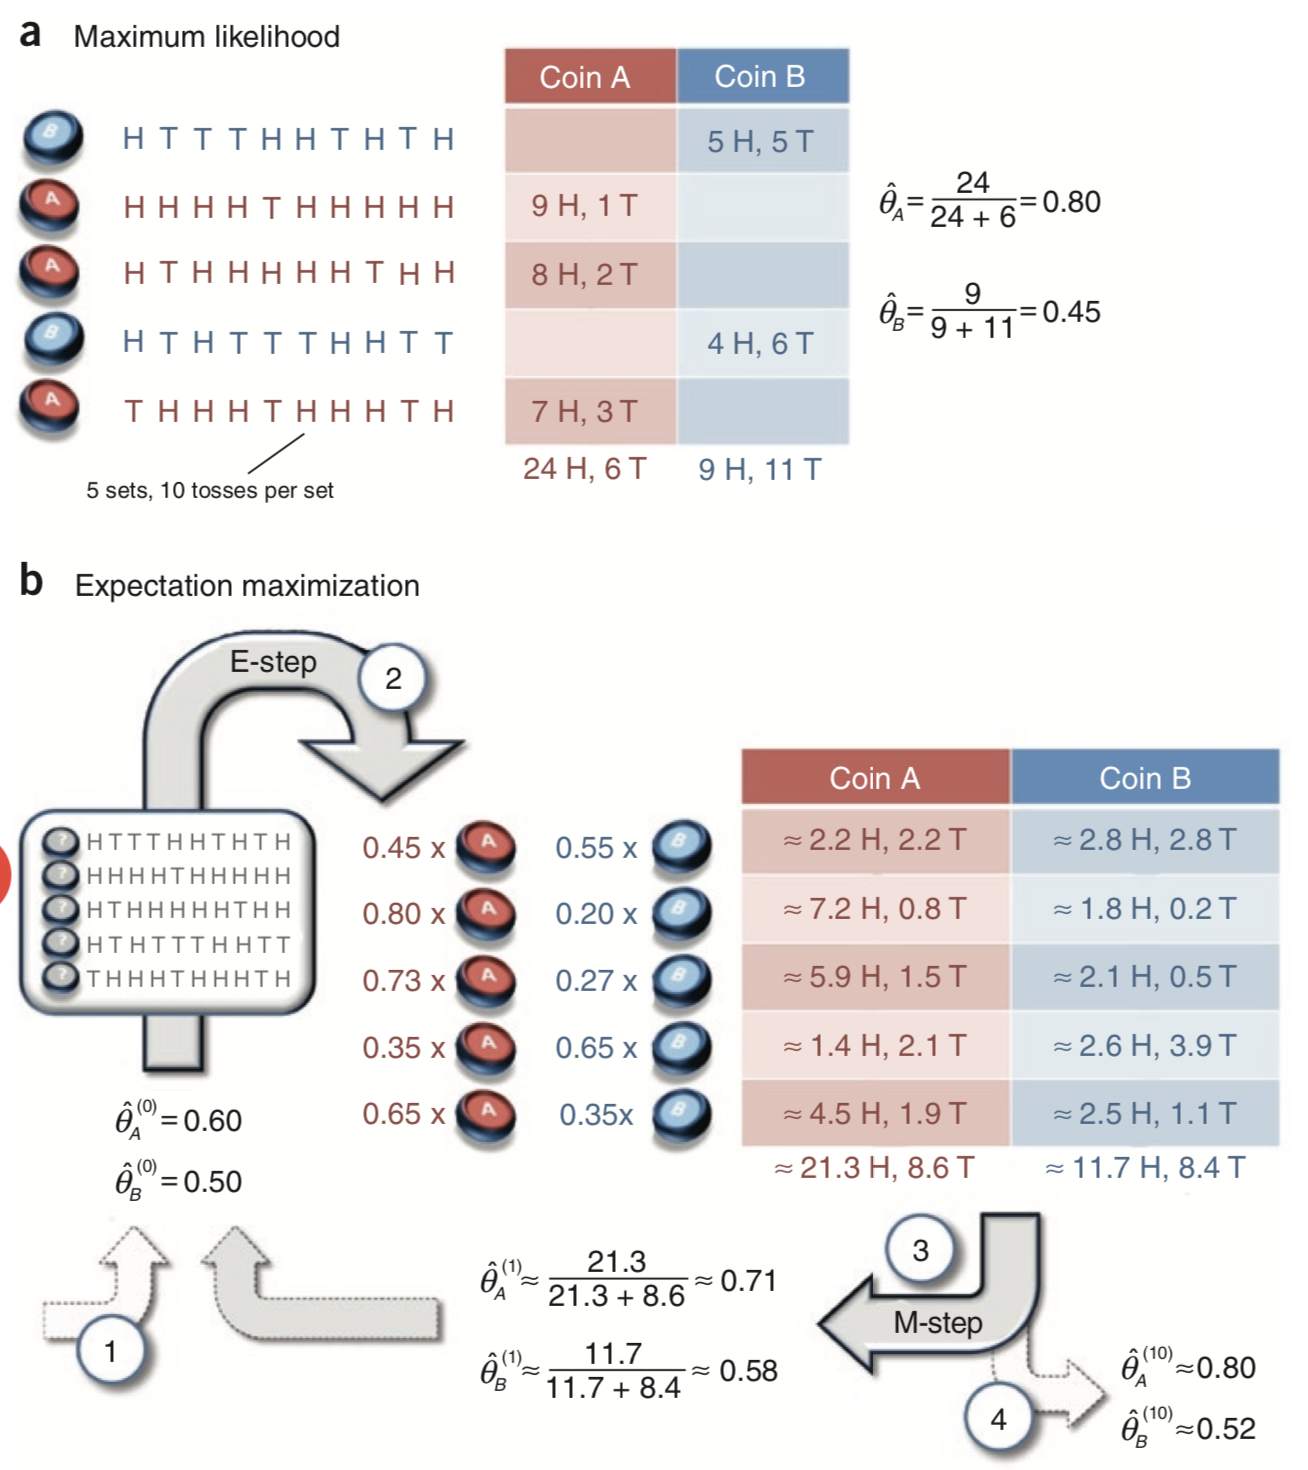
\includegraphics[width=0.5\columnwidth]{example.png} % Example image
	\caption{Example: As an example, consider a simple coin-flipping experiment in which we are given a pair of coins A and B of unknown biases, $\theta_A$ and $\theta_B$, respectively. Our goal is to estimate $\theta = (\theta_A, \theta_B)$ by repeating the following procedure five times: randomly choose one of the two coins (with equal probability), and perform ten independent coin tosses with the selected coin. Thus, the entire procedure involves a total of 50 coin tosses'}
\end{figure}

If we can figure out whether the coin we flipped is A or B, we can estimate $\theta_A$ and $\theta_B$ through one of our most familiar friends, \textbf{MLE}.(Figure 1.1a) But actually, since we can not figure it out, MLE will not work in this situation. Then EM algorithm come on the stage. EM algorithm is simple because it just contain two steps in the Iteration and EM algorithm is complex is complex for its mathematical proof and further stretch in theory and application (Figure 1.1b) andI will explain the two steps in the following section.

\subsection{Two steps in iteration of EM}
\textbf{Notation:} Given the statistical model which generates a set X of observed data(50 samples in coin-flipping experiment), a set of unobserved latent data or missing values Z(the coin is A or B), and a vector of unknown parameters $\theta$, along with a likelihood function $L(\theta; X, Z) = p(X, Z| \theta)$,  and the marginal likelihood function of the observed data is given by:

$$L(\theta; X) = p(X| \theta) = \int p(X, Z| \theta)dZ$$

However, this quantity is often intractable (we don't know the coin we tossed is A or B). 

Then the EM algorithm seeks to find the MLE of the marginal likelihood by iteratively applying the following two steps.

\textbf{(a) Expectation Step:} Define $Q(\theta| \theta^{(t})$ as the expected value of the log likelihood function of $\theta$, with respect to the current conditional distribution of Z given X and the current estimates of the parametrers $\theta^{(t)}$:

$$Q(\theta|\theta^{(t)}) = E_{Z|X,\theta^{(t)}}[logL(\theta; X, Z)] = \int P(Z|X, \theta^{(t)}) ln P(X, Z| \theta)dz $$

\textit{note:} In discrete situation, we replace $\int$ by $\sum$.  In the coin-flipping experiment, we assume $\theta^{(0)} = (\theta_A^{(0)}, \theta_B^{(0)}) = (0.60, 0.50)$. Since the results of the first ten independent tosses is X = 5 ({H: 5, T: 5}), we have $P(Z = A, X_1=5, \theta^{(0)}) = 0.6^5 \cdot 0.4^5$ and $P(Z = B, X_1=5, \theta^{(0)}) = 0.5^{10}$. Further,

$$P(Z = A|X = 5, \theta^{(0)}) = \frac{P(Z = A, X=5, \theta^{(0)})}{P(Z = A, X=5, \theta^{(0)}) + P(Z = A, X=5, \theta^{(0)})} \approx 0.45,$$ 

$$P(Z = B|X = 5, \theta^{(0)}) = \frac{P(Z = B, X=5, \theta^{(0)})}{P(Z = B, X=5, \theta^{(0)}) + P(Z = A, X=5, \theta^{(0)})} \approx 0.55$$




%----------------------------------------------------------------------------------------

\end{document}
